\documentclass{article}
\usepackage{graphicx} 
\usepackage{tikz}
\begin{document}

\title{\vspace{-70pt}\begingroup  
    \centering
    \large Grado en Intelixencia Artificial\\
    \large Sistemas Multiaxente\\[0.5em]
    \large \textbf{Práctica 1: Mundo virtual y comportamiento~individual}\par 
    \vspace{20}
    \includegraphics[width=0.6\textwidth]{mapa.png}\\
\endgroup}
\author{Pablo Chantada Saborido \\ José Romero Conde \\ Grupo del martes}

\date{}
\maketitle
\vspace{-30pt}

\newpage
\section*{\large Mundo Virtual}

El mapa consta de:
\begin{itemize}
	\item  \textbf{Pasillos:} largos y estrechos y anchos y cortos. Se busco la variedad para ofrecer un juego más interesante y probar la generalidad de los agentes.
	\item  \textbf{Pequeñas ``puertas":} aportan interés dada la sensórica de los agentes (pueden ver a través de ellas y si los escuvhan al otro lado del pasillo pueden usarlas para atraparlos.) 
\item \textbf{Escaleras y desniveles:} dan al mapa una mayor variedad. Suponen más lugares en los que se puede escapar o quedarse atrapado. 
\end{itemize}
\texttt{Resaltad los aspectos más relevantes de vuestro mundo virtual, como decisiones sobre el diseño de habitaciones, pasillos, puertas u otros elementos clave. \\ Si deseáis participar en la competición al mejor entorno, debéis incluir una imagen de vuestro escenario.}

\section*{\large Arquitectura individual}

Nuestro agente es un agente con estados, de esta forma los perceptos pasados influyen en las acciones presentes (a continuación se presenta un diagrama de estados que resume el comportamiento del agente). 

\begin{center}
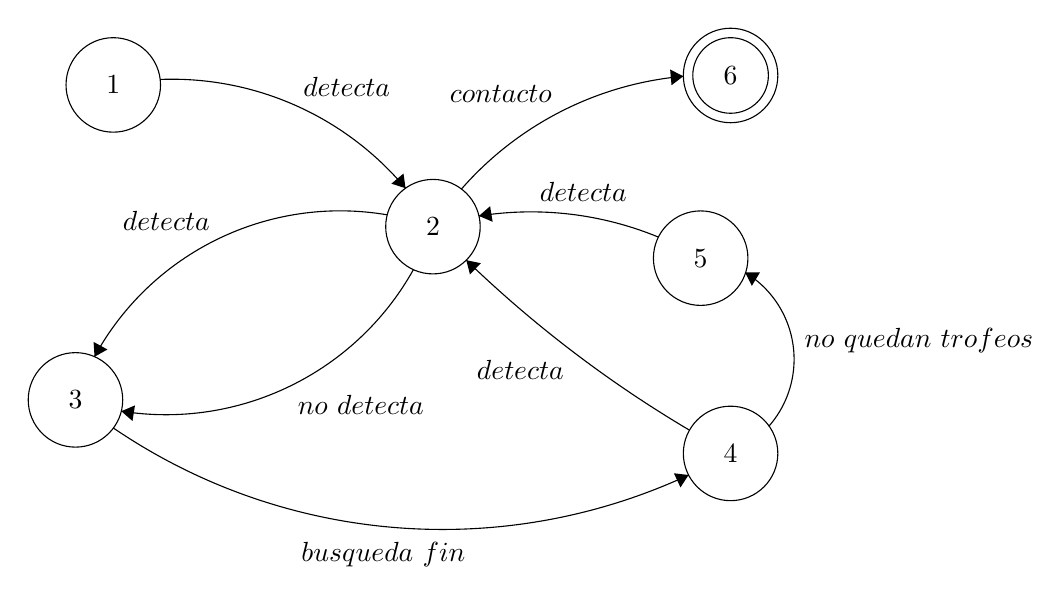
\begin{tikzpicture}[scale=0.2]
\tikzstyle{every node}+=[inner sep=0pt]
\draw [black] (18,-19.1) circle (3);
\draw (18,-19.1) node {$1$};
\draw [black] (38.3,-28.1) circle (3);
\draw (38.3,-28.1) node {$2$};
\draw [black] (15.6,-39.1) circle (3);
\draw (15.6,-39.1) node {$3$};
\draw [black] (57.2,-18.5) circle (3);
\draw (57.2,-18.5) node {$6$};
\draw [black] (57.2,-18.5) circle (2.4);
\draw [black] (57.2,-42.5) circle (3);
\draw (57.2,-42.5) node {$4$};
\draw [black] (55.3,-30.1) circle (3);
\draw (55.3,-30.1) node {$5$};
\draw [black] (20.977,-18.752) arc (92.22918:39.95064:19.345);
\fill [black] (36.56,-25.66) -- (36.43,-24.73) -- (35.66,-25.37);
\draw (32.82,-19.86) node [above] {$detecta$};
\draw [black] (16.808,-36.358) arc (151.38812:80.31982:17.773);
\fill [black] (16.81,-36.36) -- (17.63,-35.9) -- (16.75,-35.42);
\draw (21.37,-28.36) node [above] {$detecta$};
\draw [black] (37.06,-30.828) arc (-29.22438:-99.06768:18.004);
\fill [black] (18.51,-39.82) -- (19.22,-40.44) -- (19.38,-39.45);
\draw (33.72,-38.77) node [below] {$no\mbox{ }detecta$};
\draw [black] (40.11,-25.71) arc (138.80988:95.04548:21.206);
\fill [black] (54.2,-18.55) -- (53.36,-18.12) -- (53.45,-19.12);
\draw (42.61,-20.25) node [above] {$contacto$};
\draw [black] (58.129,-31.013) arc (58.77555:-41.35268:6.444);
\fill [black] (58.13,-31.01) -- (58.55,-31.86) -- (59.07,-31);
\draw (61.86,-35.35) node [right] {$no\mbox{ }quedan\mbox{ }trofeos$};
\draw [black] (54.589,-41.023) arc (-120.61879:-133.98911:76.523);
\fill [black] (40.42,-30.23) -- (40.65,-31.14) -- (41.34,-30.42);
\draw (43.85,-36.53) node [below] {$detecta$};
\draw [black] (41.22,-27.422) arc (99.014:67.56633:21.173);
\fill [black] (41.22,-27.42) -- (42.09,-27.79) -- (41.93,-26.8);
\draw (47.85,-26.51) node [above] {$detecta$};
\draw [black] (54.534,-43.873) arc (-65.06799:-124.27689:37.092);
\fill [black] (54.53,-43.87) -- (53.6,-43.76) -- (54.02,-44.66);
\draw (35.15,-48.1) node [below] {$busqueda\mbox{ }fin$};
\end{tikzpicture}
\end{center}

\begin{itemize}
	\item \textbf{1: Inicio.} patrullar en unos puntos fijos. Tarea de mantenimiento (se mantiene la hipótesis de que el ladrón no está por ahí).
	\item \textbf{2: Persecución.} Tarea de logro (se debe lograr el alcanzarlo).
	\item \textbf{3: Ir al último estado donde lo vio y patrullar ahí.} Tarea de logro (llegar al objetivo).
\item \textbf{4: Ir a los últimos trofeos que quedan y patrullar ahí.} Tarea compuesta de una parte de logro (llegar hasta los trofeos) y una de mantenimiento (que el ladrón no los consiga). Adicionalmente, si el trofeo en particular que se estaba patrullando desaparece (lo robó el ladrón), pero sigue habiendo trofeos, el agente irá a patrullar los trofeos restantes. Siendo por tanto un comnpromiso de mente abierta (no se aferrará al deseo de patrullar un trofeo que no existe).
\item \textbf{5: Ir a la salida y patrullar ahí.} Tarea compuesta de una parte de logro (llegar hasta la salida) y una de mantenimiento (que el ladrón no salga). 
\item \textbf{6: Has tocado al Ladrón.} Ganas la partida.
\end{itemize}


Como en cualquier momento puede pasar de no ver a ver al  ladrón, y eso supondrá un cambio de estado (acciones), podemos decir que el agente es audaz.

Por la forma en la que se ha presentado hasta ahora la arquitectura  del agente (Autómata de estados Finitos), esta es de subsunción.

No es, en cambio, híbrido porque aunque sí existe una representación simbólica del mundo (los estados), la acción que sucede a un percepto y un estado está completamente determinada y el agente no razona de ninguna forma. Esta decisión se basa en la hipótesis de que el mundo es suficientemente conocido de antemano como para no necesitar que el agente razone y que, solo al obedecer ordenes su comportamiento será bueno.

Toda la explicación precedente fue relativa al Policia, el ladrón, al ser jugado por el usuario humano \footnote{Para moverse, WASD; para ampliar la visión, espacio y para caminar sigilosamente (más lento pero sin ser escuchado) SHIFT.}, no lo consideramos aquí.

\texttt{Presentad una breve justificación de la arquitectura utilizada en cada uno de vuestros agentes (reactiva, deliberativa, híbrida, BDI, etc.), explicando las razones de vuestra elección.}
\section*{\large Sensores}
\begin{center}{ \includegraphics[width=0.4\textwidth]{vision.png}}\end{center}\\
\begin{itemize}
	\item \textbf{Vista:} el agente cuenta con un cono de visión que le permite ver a una cierta distancia de él con un cierto ángulo con respecto a la normal. No le permite en cambio, ver a través de las paredes.
	\item \textbf{Oído:} el agente cuenta con un radio de audición, aquello que suene dentro de esta región será percibido por el agente. Acompañamos esta habilidad sensórica del agente con la posibilidad de que el Ladrón haga o no ruído.
\end{itemize}

\texttt{Describid y justificad la elección de cada uno de los sensores que habéis decidido incluir, explicando su función y relevancia dentro del sistema.}
\section*{\large Actuadores}
\begin{itemize}
	\item \textbf{Movimiento:} el agente puede moverse bajo dos circunstancias, está dirigiendose a un punto de interés particular o esta patrullando. Naturalmente la cualidad de ``interes" de un punto es ignorada por el agente y para el siempre se esta dirigiendo a puntos igual de importantes. No obstante, no siempre avanza con la misma velocidad, si está persiguiendo se desplaza a  1.5 veces más rápido y si protege al tesoro 1.2.
	\item \textbf{Tacto:} el agente perseguirá al ladrón y cuando este lo suficientemente cerca, lo tocará para ganar la partida.
\end{itemize}
\texttt{Describid y justificad la elección de cada uno de los actuadores que habéis decidido incluir, explicando su función y relevancia dentro del sistema.}
\end{document}
